\section{Test Case Data Characteristics in Longwave region}
%==========================================================
\subsection{IASI Data}
%---------------------
The sampling characteristics of a section of the band 1 IASI data for a GDAS test case is shown in figure \ref{fig:iasi_characteristics}. Comparing the IASI sample size plot to that for AIRS in figure \ref{fig:airs_characteristics} show much more variation in the 720-760\invcm{} region. In addition, the lower panel of figure \ref{fig:iasi_characteristics} shows that the IASI subset channel selection is more diverse than that for AIRS in that both on- and off-line channels are included. 
\begin{figure}[htp]
  \centering
  \includegraphics[bb=70 340 540 571,clip,scale=0.8]{graphics/iasi_characteristics.eps}
  \caption{Characteristics of QC'd IASI data highlighting the NESDIS and EUMETSAT channel subsets used for NWP data assimilation. \textbf{(Upper panel)} Sample size of IASI data that made it past quality control. \textbf{(Lower panel)} Sample IASI spectrum indicating where the various subset channels occur.}
  \label{fig:iasi_characteristics}
\end{figure}
Comparison of the IASI sample size plot with the spectrum in figure \ref{fig:iasi_characteristics} indicates the spectral structure in the channel subset is the reason for the variation in the sample size from 720-760\invcm{}. The EUMETSAT channel set for IASI includes more on-line channels. These channels peak higher in the atmosphere and are thus less affected by the surface, and less likely to cloud affected; thus more data is retained. The NESDIS channel set for IASI includes predominantly off-line channels (somewhat similar to AIRS). These channels peak lower in the atmosphere an thus are more likely to include surface and/or cloud effects; thus more data is discarded.

\subsection{AIRS Data}
%---------------------
The sampling characteristics module 11 and 10 AIRS data for a GDAS test case is shown in figure \ref{fig:airs_characteristics}. The area of interest is the 720-760\invcm{} spectral region which is quite smooth in the upper panel of the figure. Also note that the subset channels superimposed on sample AIRS spectra in the lower panel of figure \ref{fig:airs_characteristics} indicate that predominantly off-line channels were selected in this region.
\begin{figure}[htp]
  \centering
  \includegraphics[bb=70 340 540 571,clip,scale=0.8]{graphics/airs_characteristics.eps}
  \caption{Characteristics of QC'd AIRS data highlighting the channel subset used for NWP data assimilation. \textbf{(Upper panel)} Sample size of AIRS data that made it past quality control. \textbf{(Lower panel)} Sample AIRS spectra indicating where the various subset channels occur.}
  \label{fig:airs_characteristics}
\end{figure}


\subsection{Conclusion}
%----------------------
The CompactOPTRAN fitting statistics for both IASI and AIRS do not show significant differences between the on- and off-line channels. Thus, it is unlikely that the variation seen in the sample size plots for IASI are due to a problem with the CRTM. The differences in the type of channel subsets for IASI compared to AIRS indicates that the sample size variations are physically meaningful features due to the differences in height at which the on- and off-line channel senstivities occur.

